\documentclass[12pt]{article}

\usepackage[margin=1in]{geometry} 
\usepackage{amsmath,amsthm,amssymb}
\usepackage{graphicx}
\usepackage{bm}
\usepackage[normalem,normalbf]{ulem}

\usepackage{tikz}
\usetikzlibrary{shapes.symbols}
\newcommand*\circled[1]{\tikz[baseline=(char.base)]{
		\node[shape=circle,draw,inner sep=2pt] (char) {#1};}}

\newcommand{\N}{\mathbb{N}}
\newcommand{\Z}{\mathbb{Z}}
\newcommand{\la}{\enskip\land\enskip}
\newcommand{\lo}{\enskip\lor\enskip}

\DeclareMathOperator{\lcm}{lcm}

\newtheorem{theorem}{Theorem}

\newenvironment{exercise}[2][Exercise]{\begin{trivlist}
		\item[\hskip \labelsep {\bfseries #1}\hskip \labelsep {\bfseries #2.}]}{\end{trivlist}}

\makeatletter
\renewcommand*\env@matrix[1][*\c@MaxMatrixCols c]{%
	\hskip -\arraycolsep
	\let\@ifnextchar\new@ifnextchar
	\array{#1}}
\makeatother



\begin{document}
	
	% --------------------------------------------------------------
	%                         Start here
	% --------------------------------------------------------------
	
	
	\title{Homework 1 (Due Jan 18, 2023)}
	\author{Jack Hyatt\\ %replace with your name
		MATH 575 - Discrete Mathamatics II - Spring 2023} 
	
	\maketitle
	
	Justify all of your answers completely.\\
	
	\renewcommand{\qedsymbol}{$\blacksquare$}
	
	\medskip 
	
	
	
	\begin{enumerate}


\item For positive integers $n$ and $k$, consider the graph $G(n,k)$ which is defined as follows: the vertex set of $G(n,k)$ is the set of subsets of $[n]$ of size $k$, and two vertices are connected by an edge in $G(n,k)$ if and only if the corresponding subsets are disjoint. \footnote{ E.g., $V(G(4,2)) = \{\{1,2\},\{1,3\},\{1,4\},\{2,3\},\{2,4\},\{3,4\}\}$ and \[E(G(4,2)) = \{\{\{1,2\},\{3,4\}\}, \qquad \{\{1,3\},\{2,4\}\},\qquad \{\{1,4\},\{2,3\}\}\} \]}
\begin{enumerate}
\item Give a drawing of the graph $G(5,2)$. \\
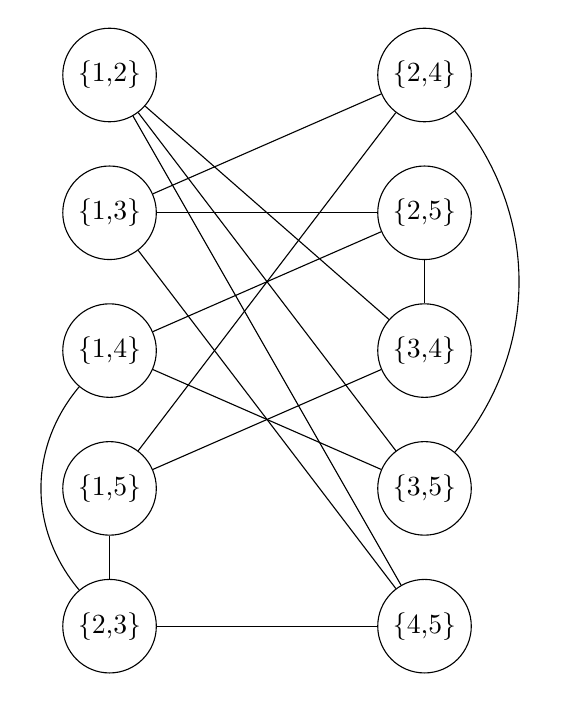
\begin{tikzpicture}[main/.style = {draw, circle}]
	\node[main] (1) {\{1,2\}};
	\node[main] (2) [below of=1,yshift=-.75cm] {\{1,3\}};
	\node[main] (3) [below of=2,yshift=-.75cm] {\{1,4\}};
	\node[main] (4) [below of=3,yshift=-.75cm] {\{1,5\}};
	\node[main] (5) [below of=4,yshift=-.75cm] {\{2,3\}};
	\node[main] (6) [right of=1,xshift=3cm] {\{2,4\}};
	\node[main] (7) [right of=2,xshift=3cm] {\{2,5\}};
	\node[main] (8) [right of=3,xshift=3cm] {\{3,4\}};
	\node[main] (9) [right of=4,xshift=3cm] {\{3,5\}};
	\node[main] (10) [right of=5,xshift=3cm] {\{4,5\}};
	\draw (1) -- (8);
	\draw (1) -- (9);
	\draw (1) -- (10);
	\draw (2) -- (6);
	\draw (2) -- (7);
	\draw (2) -- (10);
	\draw [bend right = 40] (3) to (5);
	\draw (3) -- (7);
	\draw (3) -- (9);
	\draw (4) -- (5);
	\draw (4) -- (6);
	\draw (4) -- (8);
	\draw (5) -- (10);
	\draw [bend left = 40] (6) to (9);
	\draw (7) -- (8);
\end{tikzpicture}\newpage
\item Let $G$ be the graph drawn below. Show that $G(5,2)$ is isomorphic to $G$ by relabelling the vertices of $G$ in the drawing below.
\begin{center}
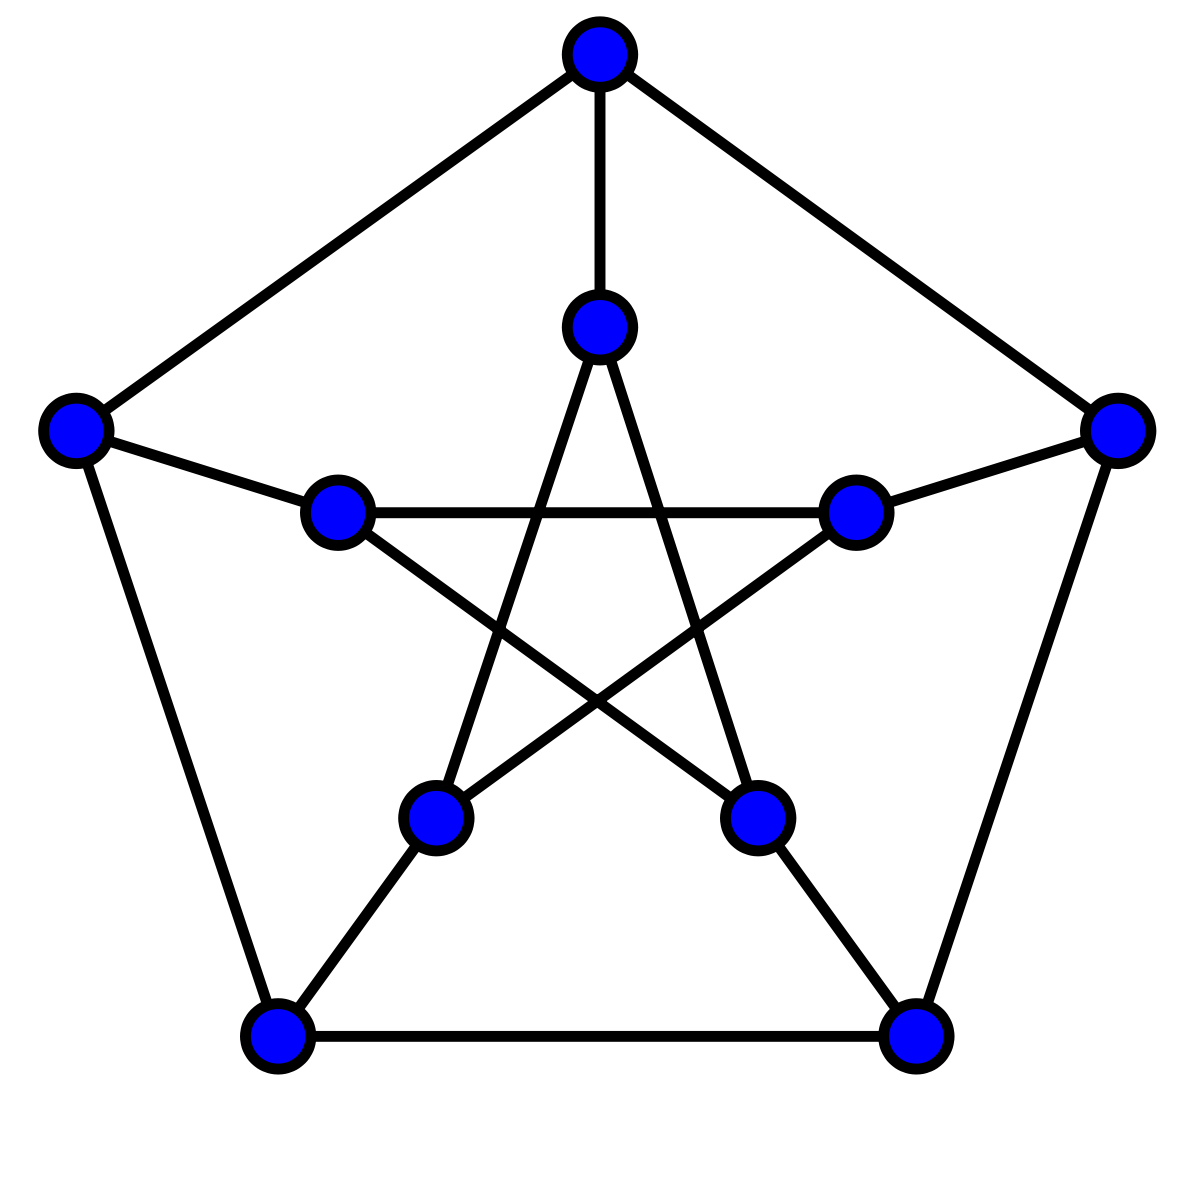
\includegraphics[scale=.1]{petersen.png}\\
Here is the labeled graph\\
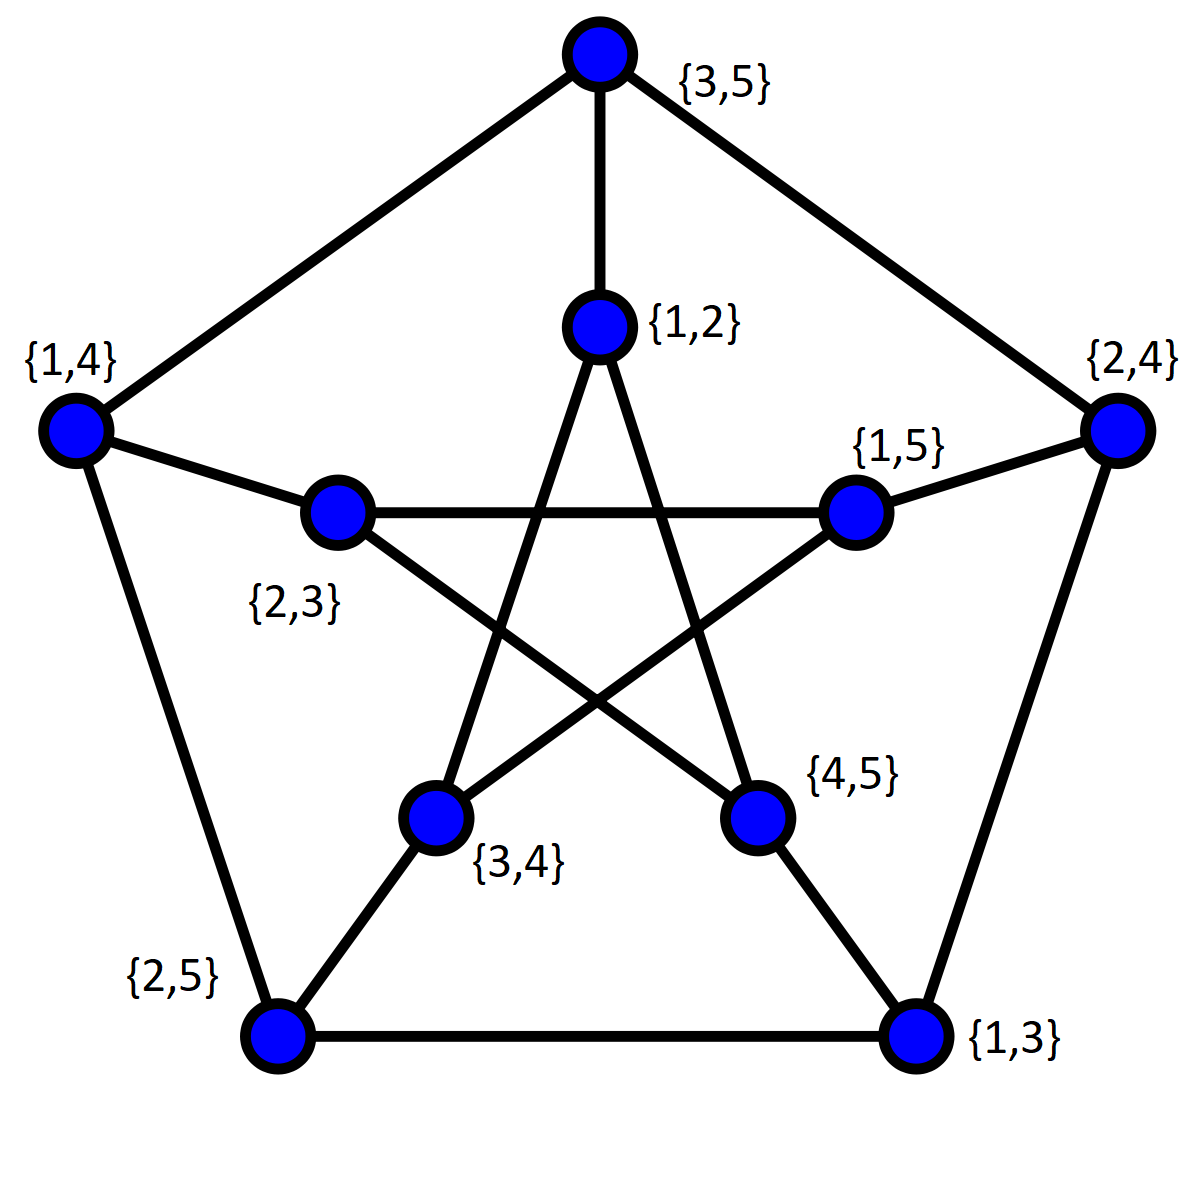
\includegraphics[scale=.25]{petersen-labeled.png}
\end{center}
\end{enumerate}


\medskip

\item A graph is called {\bf $k$-regular} if every vertex has degree $k$. 
\begin{enumerate}
\item Draw an example of a $3$-regular graph on $6$ vertices.\\
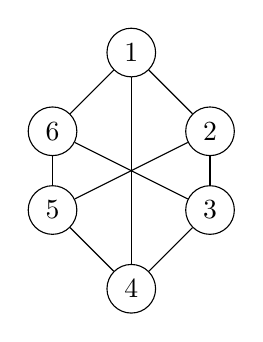
\begin{tikzpicture}[main/.style = {draw, circle}]
	\node[main] (1) {1};
	\node[main] (2) [below of=1,right of=1] {2};
	\node[main] (3) [below of=2] {3};
	\node[main] (4) [below of=3,left of=3] {4};
	\node[main] (5) [above of=4,left of=4] {5};
	\node[main] (6) [above of=5] {6};
	\draw (1)--(2);
	\draw (1)--(6);
	\draw (1)--(4);
	\draw (2)--(3);
	\draw (2)--(5);
	\draw (3)--(4);
	\draw (3)--(6);
	\draw (5)--(4);
	\draw (5)--(6);
\end{tikzpicture}
\item Draw two nonisomorphic $2$-regular graphs on $7$ vertices.\\
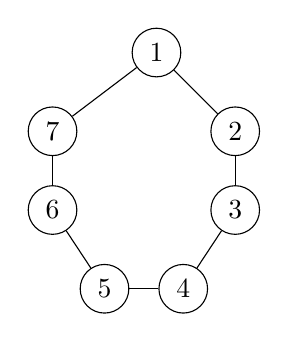
\begin{tikzpicture}[main/.style = {draw, circle}]
	\node[main] (1) {1};
	\node[main] (2) [below of=1,right of=1] {2};
	\node[main] (3) [below of=2] {3};
	\node[main] (4) [below of=3,xshift=-.66cm] {4};
	\node[main] (5) [left of =4] {5};
	\node[main] (6) [above of=5,xshift=-.66cm] {6};
	\node[main] (7) [above of=6] {7};
	\draw (1)--(2);
	\draw (2)--(3);
	\draw (3)--(4);
	\draw (4)--(5);
	\draw (5)--(6);
	\draw (6)--(7);
	\draw (7)--(1);
\end{tikzpicture}
\item Prove that if $k$ is odd, then there does not exist a $k$-regular graph with an odd number of vertices. 
\begin{proof}
	Assume we have a graph, G, that is k-regular, where k is odd. Assume towards contradiction that G has an odd number of vertices, namely n. By Handshaking lemma, summing up the degrees of the vertices will be an even number, but in G, it will be $nk$. This is an odd number multiplied by an odd number, which is not even. 
\begin{tikzpicture}
			\node[starburst, draw, minimum width=3cm, minimum height=2cm,line width=1.5pt,red,fill=yellow,scale=.5]
		{BOOM, A CONTRADICTION!!!};
	\end{tikzpicture}
\end{proof}
\end{enumerate}

\medskip

\item Prove that every graph $G$ must contain a pair of vertices with the same degree. 

\begin{proof}
	Let $v_1,v_2,...,v_n$ be the vertices of G, and $d_i$ be the degree of $v_i$. There are $n$ different possible numbers $d_i$ can be, namely $0,...,n-1$. If a vertex has a degree of $n-1$, then it is neighbors to every other vertex, making another vertex having a degree of 0 impossible. So a graph with every degree is impossible, meaning a graph can at most have $n-1$ different $d_i$'s. So by PHP, matching $n$ vertices to $n-1$ degrees must result in 2 vertices having the same degree.
\end{proof}

\medskip

\item Let $G$ be a graph with $V(G) = \{v_1, \ldots, v_n\}$. Recall that the {\em adjacency matrix} of $G$ is the $n \times n$ matrix $A$ such that $A_{ij} = 1$ if $v_iv_j \in E(G)$ and $A_{ij} = 0$ otherwise. Use induction to prove that for all integers $k \geq 1$, the $(i,j)$-entry of $A^k$ is equal to the number of $v_i,v_j$-walks of length $k$ in $G$. 
\begin{proof}
	Let us induct on the degree of adjacency matrix A.\\
	Base case: \boldsymbol{$k=1$}\\
	Obvious by the definition of adjacency matrix.\medskip\\
	Induction step: Assume that A is an adjacency matrix of G and that the $(i,j)$-entry of $A^k$ is equal to the number of $v_i,v_j$-walks of length k in G. Let us right multiply A to get $A^k\cdot A=A^{k+1}$. Looking at the $(i,j)$-entry of $A^{k+1}$, we get it from the dot product of the ith row of $A^k$ and the jth column of A. Each element in the ith row of $A^k$ is the number of walks from vertex $i$ to each intermediate vertex $q$, and those entries will be multiplied by 0 if that intermediate vertex $q$ is not adjacent to $j$. This means those walks of length $k$ starting at vertex $i$ that cannot reach $j$ by adding one more edge to the end are not added. The walks of length $k$ that do reach $j$ after adding an edge to the end of the walk are added, since the number they are being multiplied by is 1 in the jth column of $A$. So we are left with the number of walks from vertex $i$ to an intermediate vertex $q$ (walk of length $k$) to vertex $j$, which gives a walk of length $k+1$. 
	
\end{proof}

\medskip

\item Let $G$ be an $n$-vertex graph with degree sequence $(d_1, d_2, \ldots, d_n)$.
\begin{enumerate}
\item What is the degree sequence of $\overline{G}$?
\\$(n-1-d_1,n-1-d_2,\ldots,n-1-d_n)$ is the sequence.
\item A graph $G$ is called {\em self-complementary} if it is isormophic to its complement. Prove that if $G$ is self-complementary, then either $n$ or $n-1$ is divisible by 4.
\begin{proof}
	Assume G is self-complementary. This means that $|E(G)|$ is half of the total number of edges for the complete graph with the same number of vertices, since $G\cup\overline{G}=K_n$. So $|E(K_n)|=\frac{n(n-1)}{2} \implies |E(G)|=\frac{n(n-1)}{4}$. And since $|E(G)|$ is a whole number, 4 must divide $n$ or $n-1$.
\end{proof}
\item Show that for all $n$ divisible by 4, there exists a self-complementary graph on $n$ vertices. \footnote{Hint: generalize the structure of the path $P_4$.}
\begin{proof}
	The rule set for enumerated vertices: $v_iv_j$ is an edge in the graph
	\begin{enumerate}
		\item if $v_i\equiv 1 \mod 4 \la (v_j\equiv 1 \mod 4 \lor v_j\equiv 2\mod4)$
		\item if $v_i\equiv 2 \mod 4 \la (v_j\equiv 1 \mod 4 \lor v_j\equiv 3\mod4)$
		\item if $v_i\equiv 3 \mod 4 \la (v_j\equiv 2 \mod 4 \lor v_j\equiv 0\mod4)$
		\item if $v_i\equiv 0 \mod 4 \la (v_j\equiv 3 \mod 4 \lor v_j\equiv 0\mod4)$
	\end{enumerate}
	gives a self complementary graph on $4k$ vertices.\\
	We will show the above statement by inducting on $n=4k$.\\
	Base case: \boldsymbol{$k=1$}\\
	The $P_4$ graph is self-complementary.
	\begin{center}
		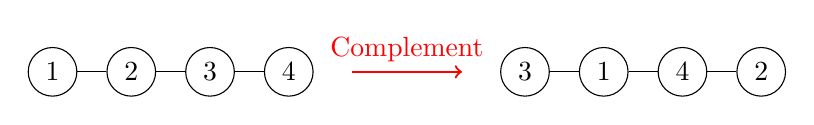
\begin{tikzpicture}[main/.style = {draw, circle}]
			\node[main] (1) {1};
			\node[main, right of=1] (2) {2};
			\node[main, right of=2] (3) {3};
			\node[main, right of=3] (4) {4};
			\draw (1)--(2);
			\draw (2)--(3);
			\draw (3)--(4);
			\node[main, right of=4,xshift=2cm] (5) {3};
			\draw [thick, ->,red] (3.8,0) -- (5.2,0) node[midway,above] {Complement};
			\node[main, right of=5] (6) {1};
			\node[main, right of=6] (7) {4};
			\node[main, right of=7] (8) {2};
			\draw (5)--(6);
			\draw (6)--(7);
			\draw (7)--(8);
		\end{tikzpicture}
	\end{center}
	\boldsymbol{$k=2$}\\
	Layering $P_4$ graphs with the rule set results in self-complementary graphs.
	\begin{center}
		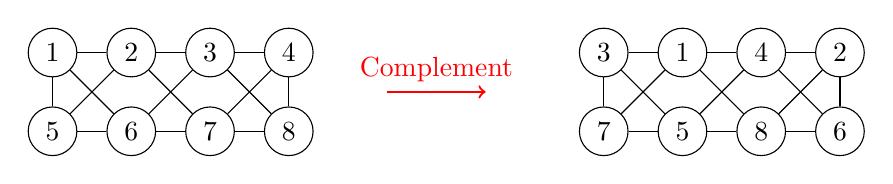
\begin{tikzpicture}[main/.style = {draw, circle}]
			\node[main] (1) {1};
			\node[main, right of=1] (2) {2};
			\node[main, right of=2] (3) {3};
			\node[main, right of=3] (4) {4};
			\draw (1)--(2);
			\draw (2)--(3);
			\draw (3)--(4);
			\node[main, below of=1] (5) {5};
			\node[main, below of=2] (6) {6};
			\node[main, below of=3] (7) {7};
			\node[main, below of=4] (8) {8};
			\draw (5)--(6);
			\draw (6)--(7);
			\draw (7)--(8);
			
			\draw (1)--(5);
			\draw (1)--(6);
			\draw (2)--(5);
			\draw (2)--(7);
			\draw (3)--(6);
			\draw (3)--(8);
			\draw (4)--(7);
			\draw (4)--(8);
			
			\draw [thick, ->,red] (4.25,-.5) -- (5.5,-.5) node[midway,above] {Complement};
			\node[main, right of=4,xshift=3cm] (11) {3};
			\node[main, right of=11] (22) {1};
			\node[main, right of=22] (33) {4};
			\node[main, right of=33] (44) {2};
			\draw (11)--(22);
			\draw (22)--(33);
			\draw (33)--(44);
			\node[main, below of=11] (55) {7};
			\node[main, below of=22] (66) {5};
			\node[main, below of=33] (77) {8};
			\node[main, below of=44] (88) {6};
			\draw (55)--(66);
			\draw (66)--(77);
			\draw (77)--(88);
			
			\draw (11)--(55);
			\draw (11)--(66);
			\draw (22)--(55);
			\draw (22)--(77);
			\draw (33)--(66);
			\draw (33)--(88);
			\draw (44)--(77);
			\draw (44)--(88);
			
			\end{tikzpicture}
	\end{center}
	\medskip
	Induction Step: Assume we have a simple graph, G, such that there are $4k$ vertices $\{v_1,\ldots,v_{4k}\}$, with the rules stated in the beginning, where $k\geq2$.
	(This is the pattern shown in base case $k=2$)\\
	Let us add 4 vertices to the graph and apply the rule to those vertices. We know from the base case $k=2$ that the subgraph of this new "layer" and any other layer will be self-complementary. Since the vertices in the new layer are self complementary with every other layer, and the other layers were already self-complementary in total, this new graph with $4(k+1)$ vertices is also self complementary.
\end{proof}
\item Show that for all $n$ such that $n-1$ is divisible by $4$, there exists a self-complementary graph on $n$ vertices. \footnote{Hint: add a vertex to a construction in part (c).}\\\\
In part (c), we constructed a graph with 4k vertices that was self-complementary. Let us add a single vertex to our graph. It is now not self-complementary. To make it self complementary, we must connect the vertex to the "outer" vertices in each "row". This makes the graph self-complementary, since the vertices our new vertex is adjacent to in the complement graph are now the "outer" vertices (i.e. 2 and 3 become the outer vertices), and we still have half the total possible edges. So now we have a self-complementary construction for every graph with n vertices where $4|(n-1)$. 
\end{enumerate}

\end{enumerate}
\end{document}
